% !TEX root = thesis.tex
\FloatBarrier
\section{Results}
\label{sec:exp}



%\subsection{Data}
%\begin{figure}[htp]
%\centering
%%\begin{subfigure}{0.95\textwidth}
%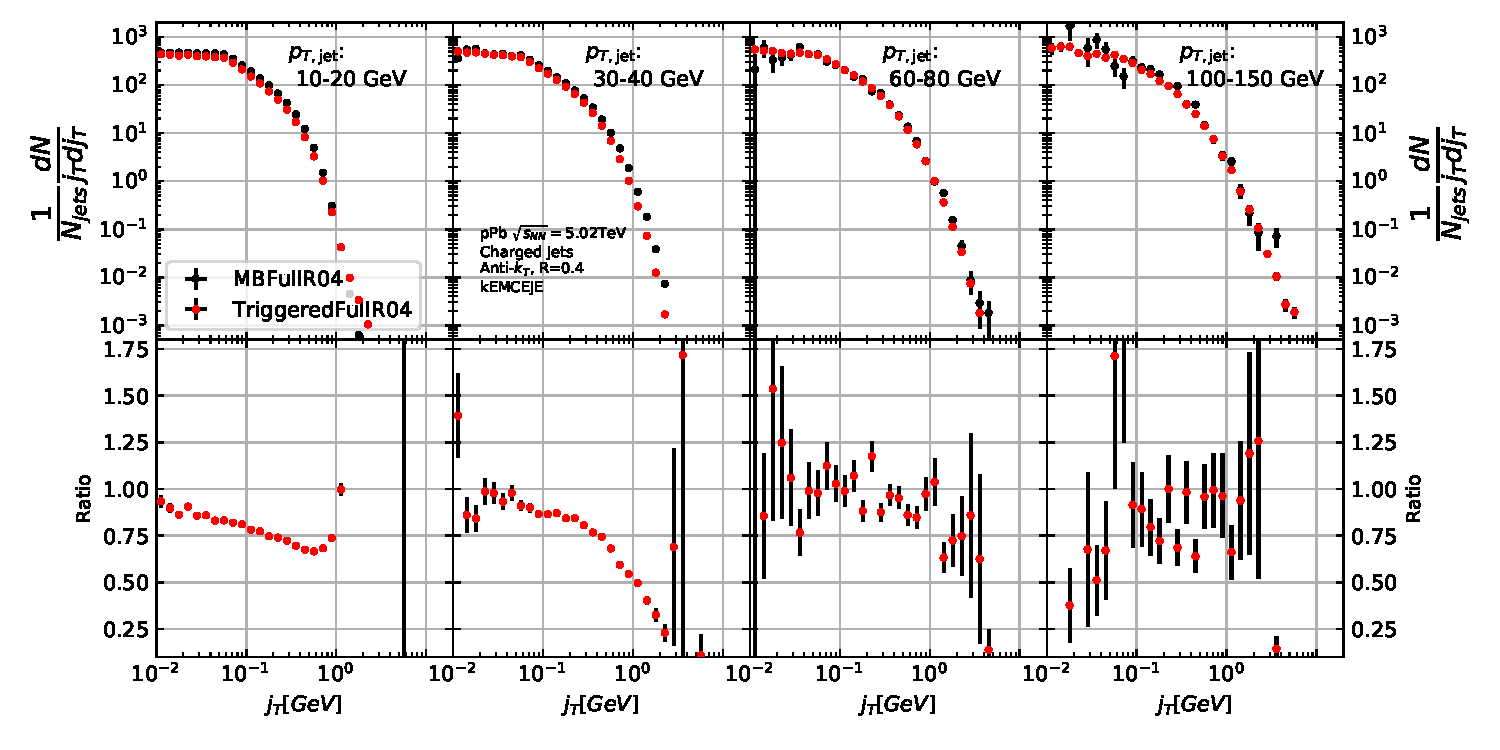
\includegraphics[width=0.95\textwidth]{results/MBvsTriggeredFullJetsR04JetConeJt.pdf} 
%%Tag 20170810 python2.7 Python/MBtoTriggeredComparison.py legotrain_CF_pPb-1053_20170223-2002_LHC13bcde.root
%
%%\includegraphics[width=0.95\textwidth]{results/OverlayjetjtIncl_T02_\figComment}
%\caption{Comparison between minimum bias and triggered datasets }
%%\end{subfigure}
%%\begin{subfigure}{0.5\textwidth}
%%%\includegraphics[width=0.95\textwidth]{results/OverlayjetjtIncl_T06_\figComment}
%%%\caption{Jet $p_T$ 80-100 GeV}
%%\end{subfigure}
%\end{figure}
%\subsection{Inclusive results}


%As outlined in Section ~\ref{sec:analysis} the inclusive $\jt{}$ distributions and corresponding backgrounds are obtained for different jet $p_T$ bins starting from $10\:\gev < \pt{jet} < 20\:\gev$. Later the lowest $\pt{}$ bins are omitted because of problems in unfolding and fitting. The results are shown in Fig.~\ref{fig:inclusive}. The background distribution the figure is obtained by the perpendicular cone method.







\subsection{Fitting}
Fits of $j_T$ distributions in different jet $p_T$ bins with $p_T  > 40 \gev$ are shown in figure \ref{fig:fits}. Additional jet $p_T$ bins are shown in appendix \ref{app:a}. In lowest jet $p_T$ bins the jets are mainly combinatorial which makes background subtraction and unfolding difficult and thus the signal can't be trusted. 

The fits describe the data well. There is some fluctuation of the order of 10 \% around the fit function. At hight $j_T$ the statistical errors in the signal are large.

\begin{figure}
\centering
%\begin{subfigure}{0.24\textwidth}
%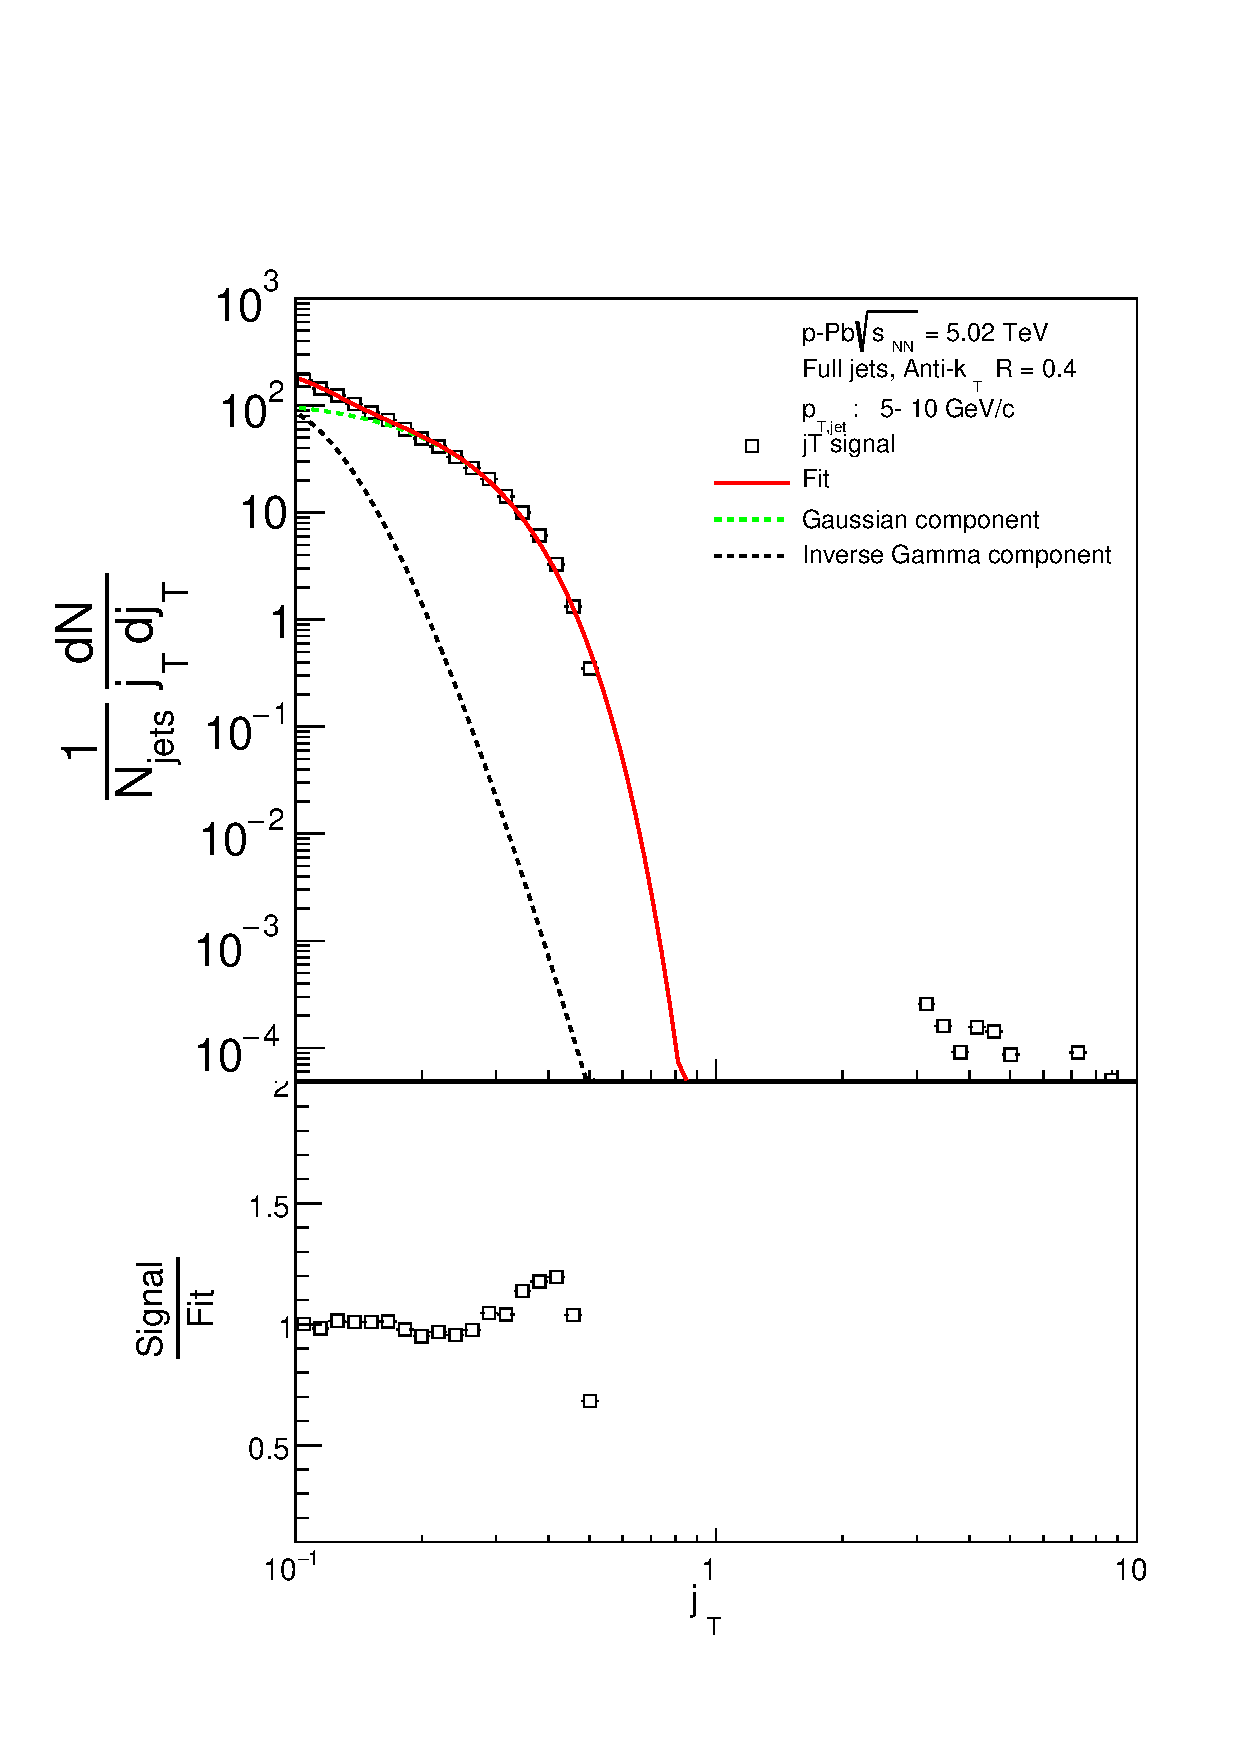
\includegraphics[width=0.95\textwidth]{RooUnfold/figs/JetConejTSignalFit/JetConejTSignalFitNFin00JetPt00perconeBgBayes}
%\end{subfigure}
%\begin{subfigure}{0.24\textwidth}
%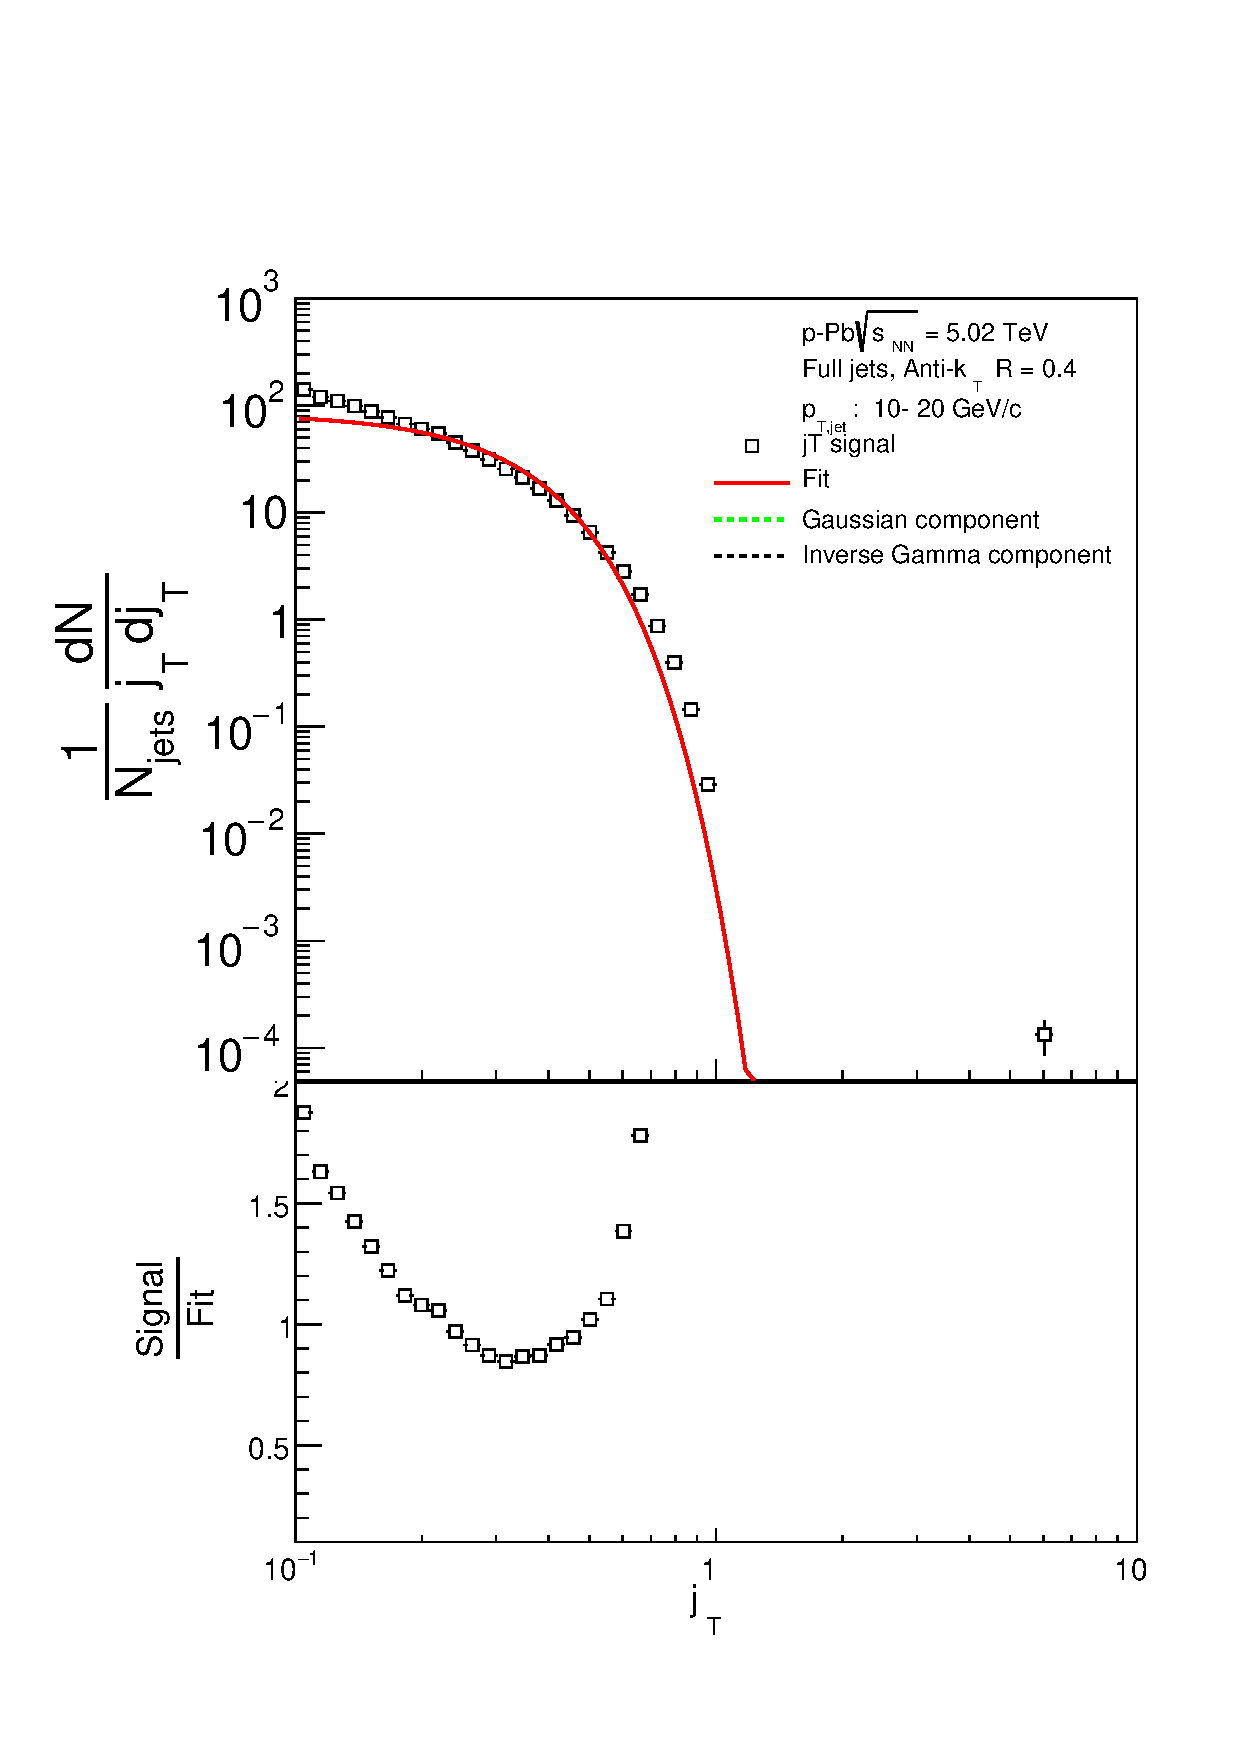
\includegraphics[width=0.95\textwidth]{RooUnfold/figs/JetConejTSignalFit/JetConejTSignalFitNFin00JetPt01perconeBgBayes}
%\end{subfigure}
%\begin{subfigure}{0.24\textwidth}
%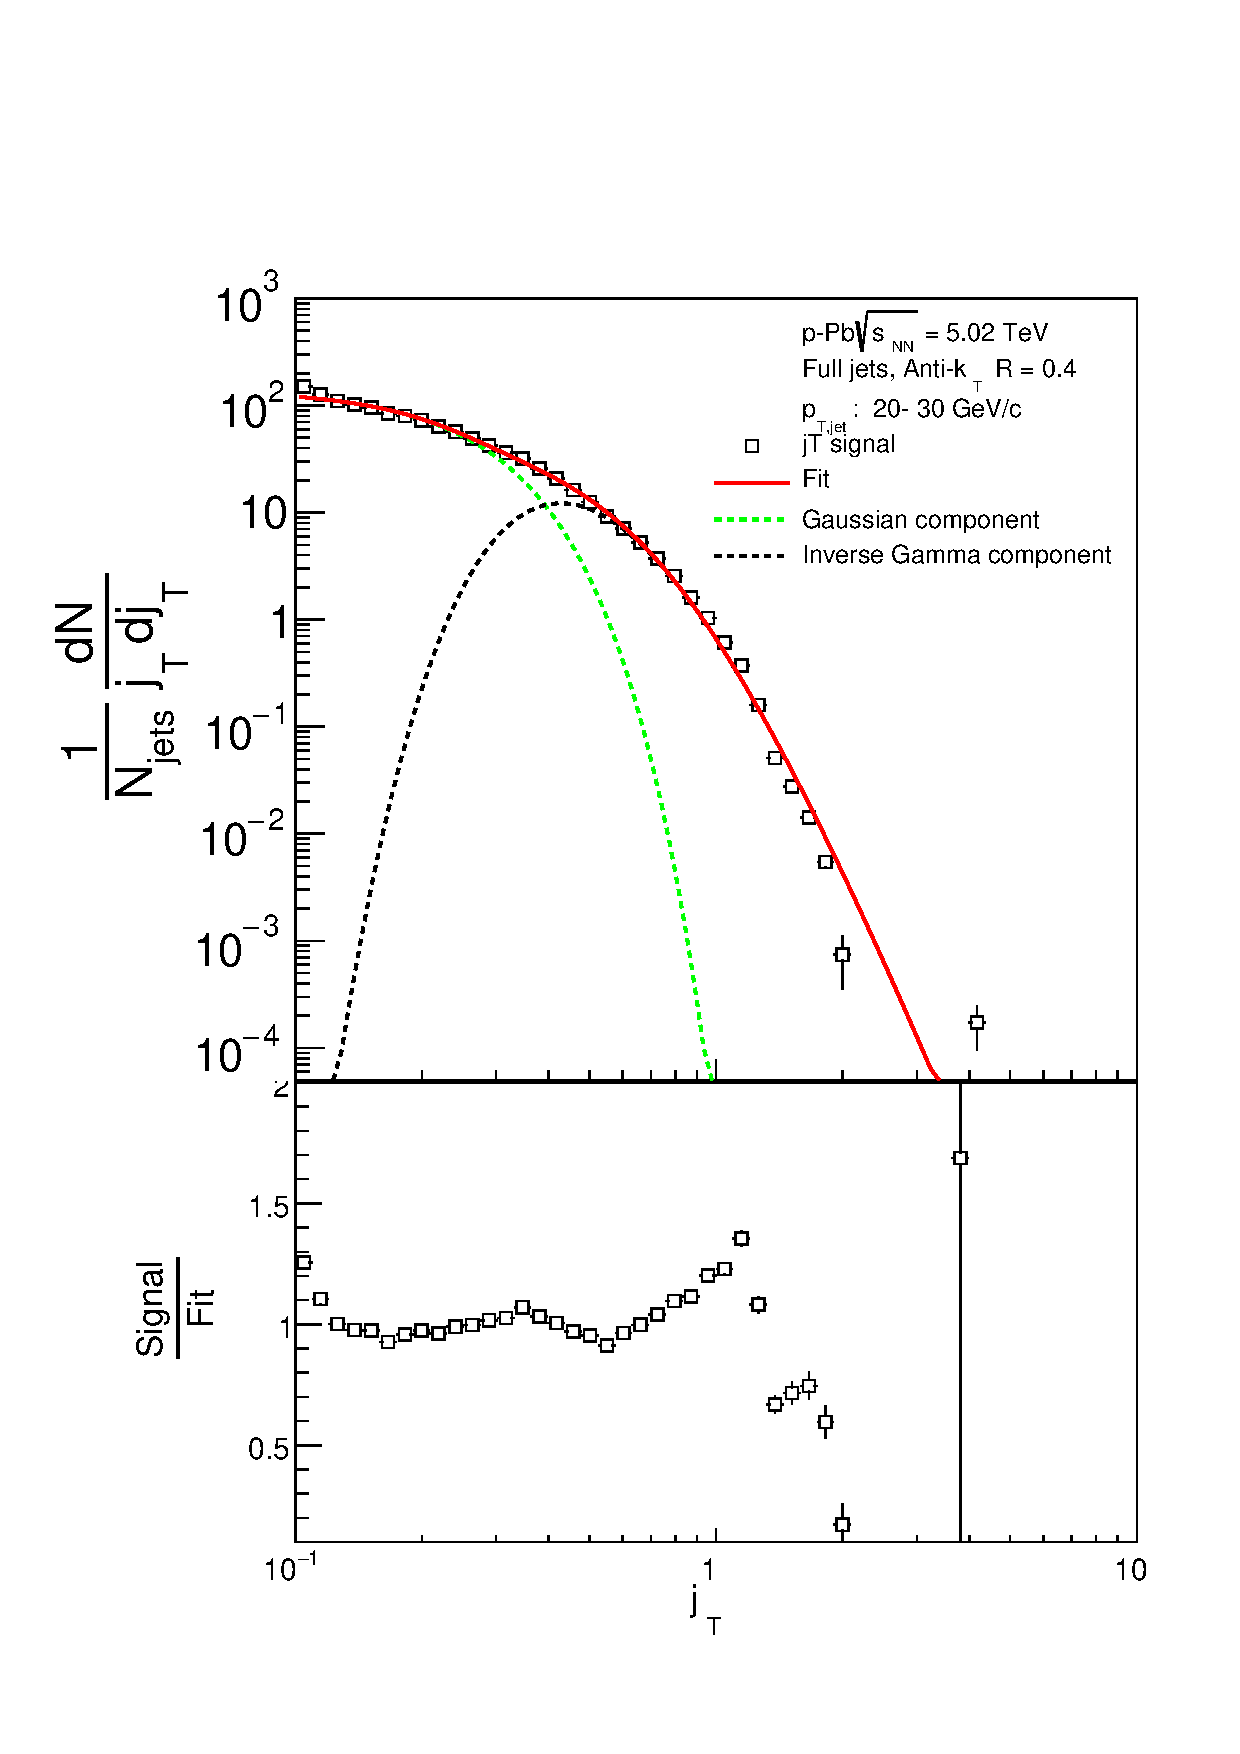
\includegraphics[width=0.95\textwidth]{RooUnfold/figs/JetConejTSignalFit/JetConejTSignalFitNFin00JetPt02perconeBgBayes}
%\end{subfigure}
%\begin{subfigure}{0.24\textwidth}
%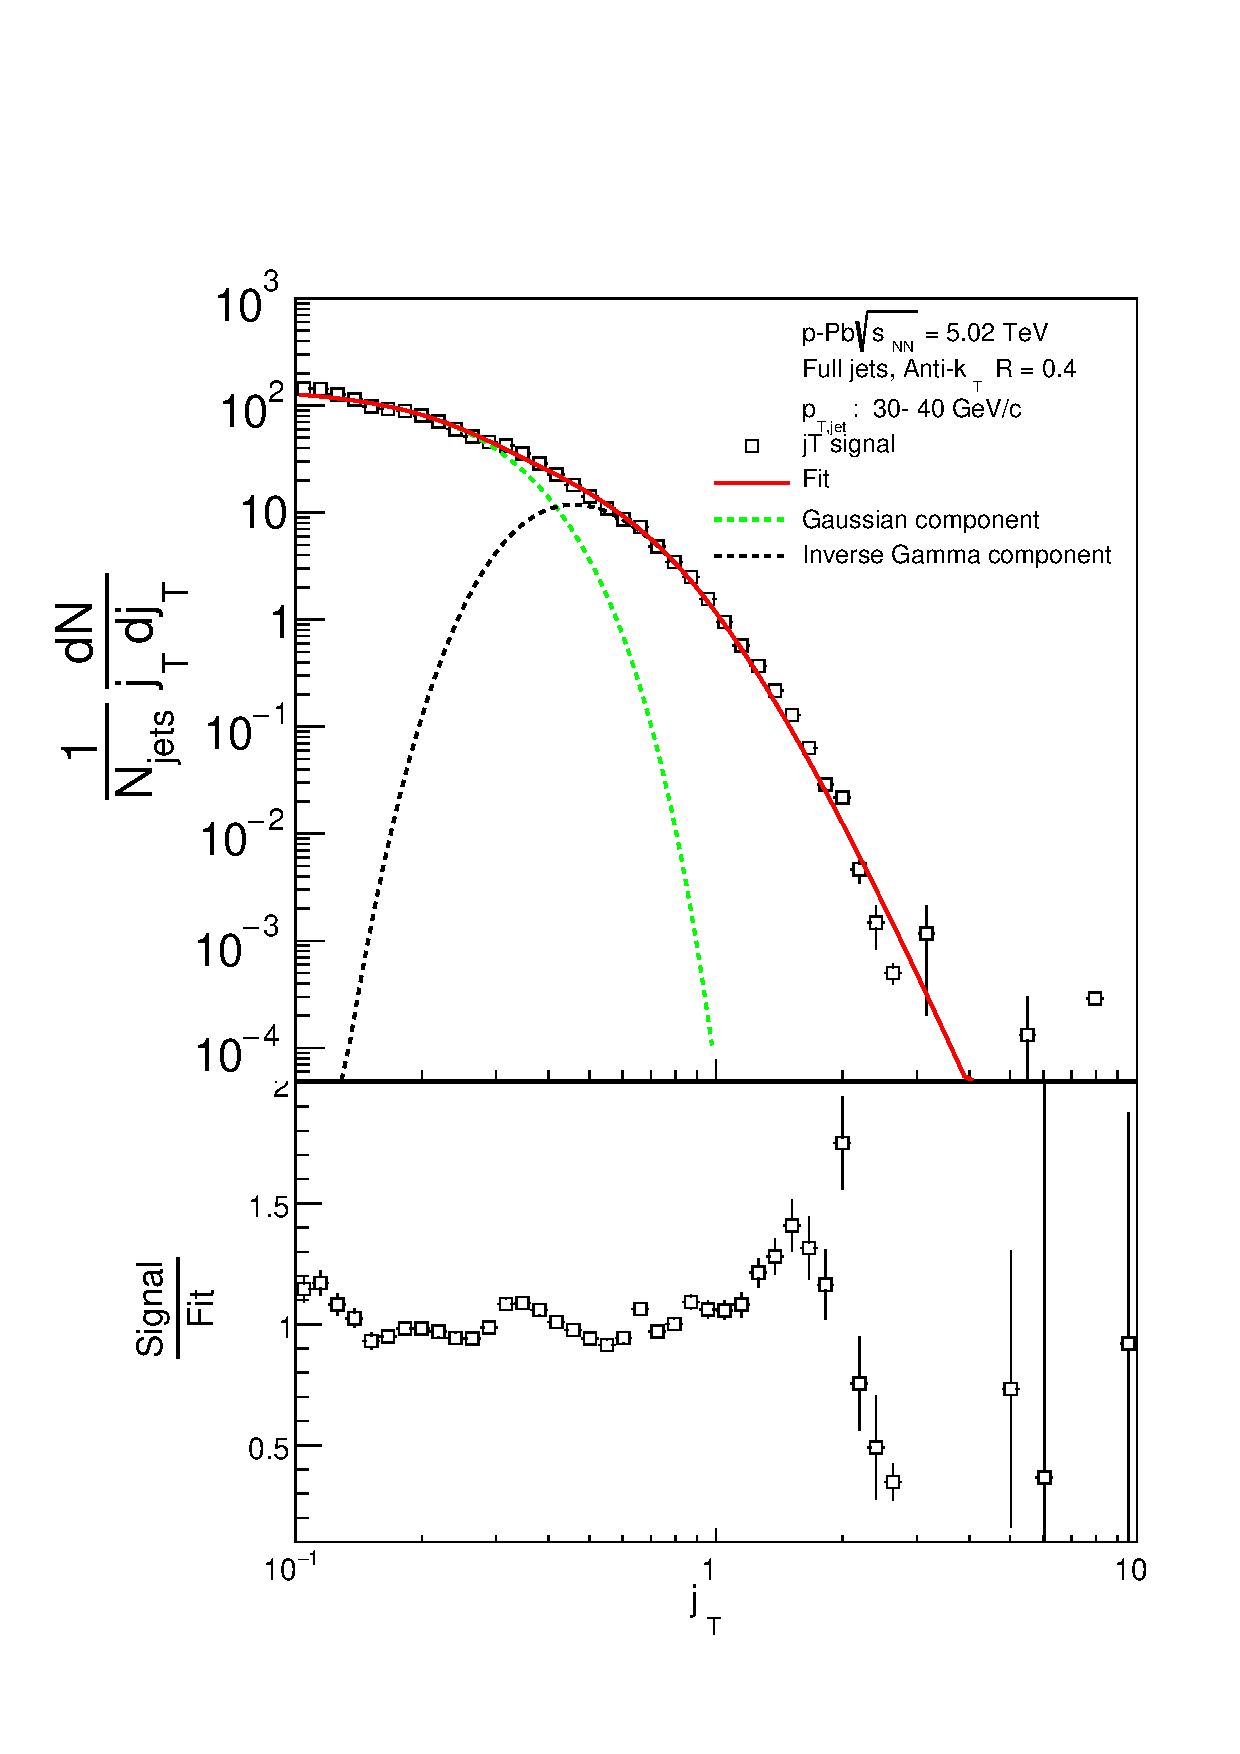
\includegraphics[width=0.95\textwidth]{RooUnfold/figs/JetConejTSignalFit/JetConejTSignalFitNFin00JetPt03perconeBgBayes}
%\end{subfigure}
\begin{subfigure}{0.24\textwidth}
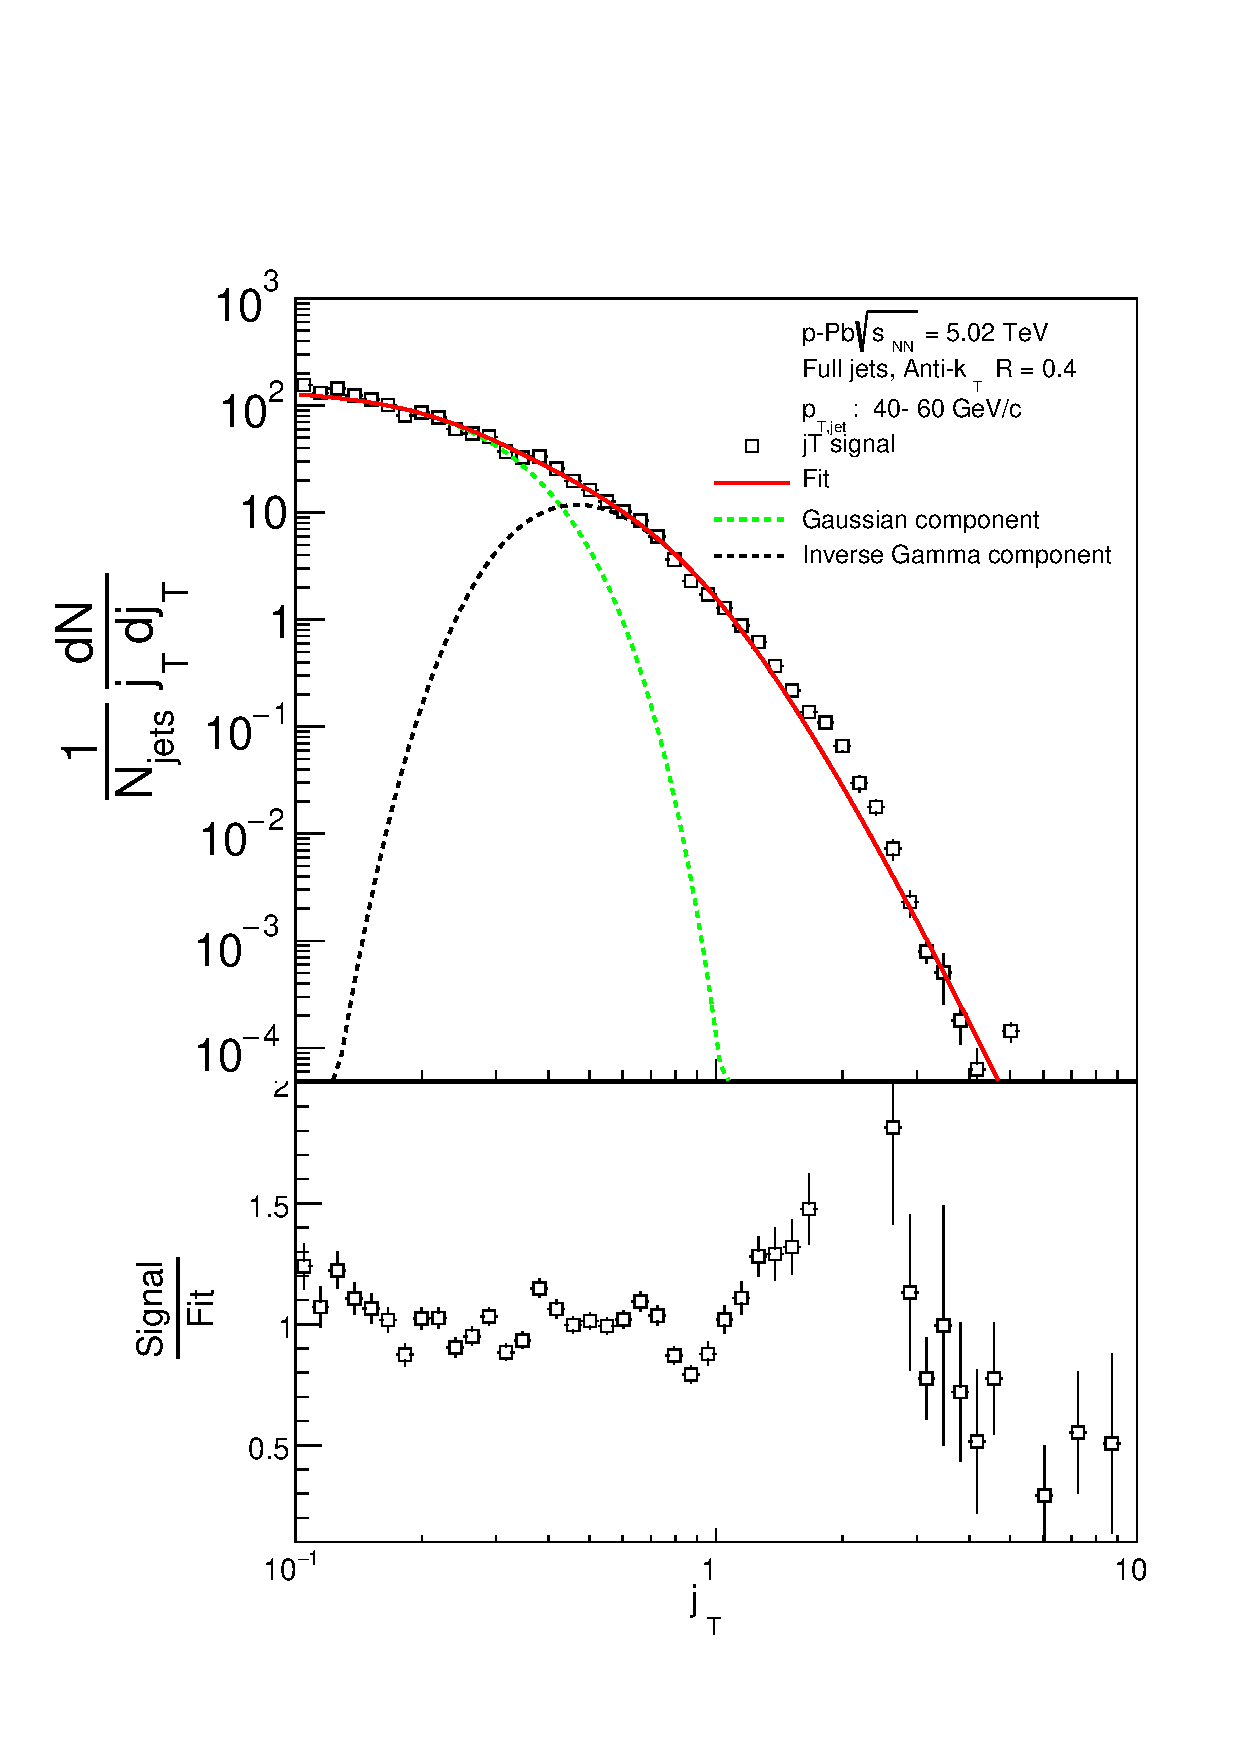
\includegraphics[width=0.95\textwidth]{results/JetConejTSignalFit/JetConejTSignalFitNFin00JetPt04perconeBgBayes}
\end{subfigure}
\begin{subfigure}{0.24\textwidth}
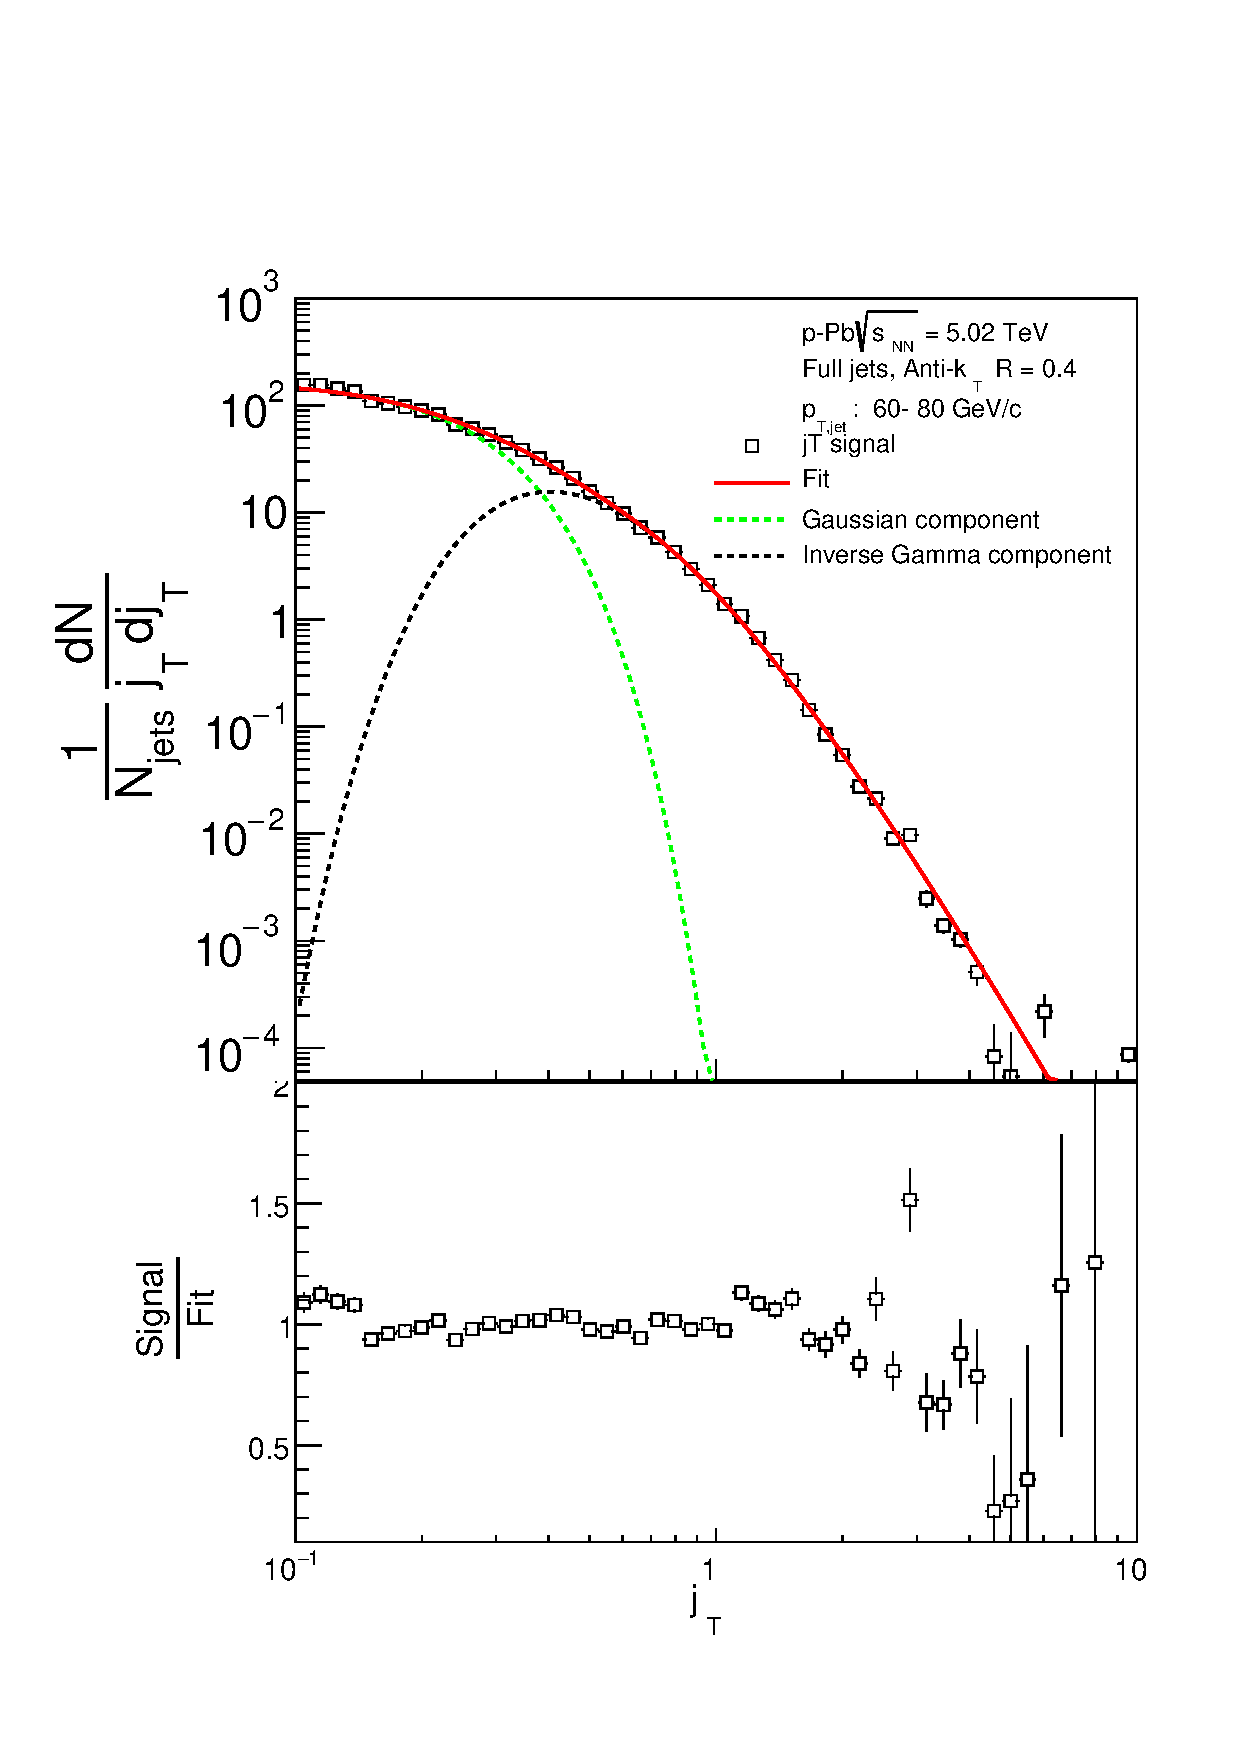
\includegraphics[width=0.95\textwidth]{results/JetConejTSignalFit/JetConejTSignalFitNFin00JetPt05perconeBgBayes}
\end{subfigure}
\begin{subfigure}{0.24\textwidth}
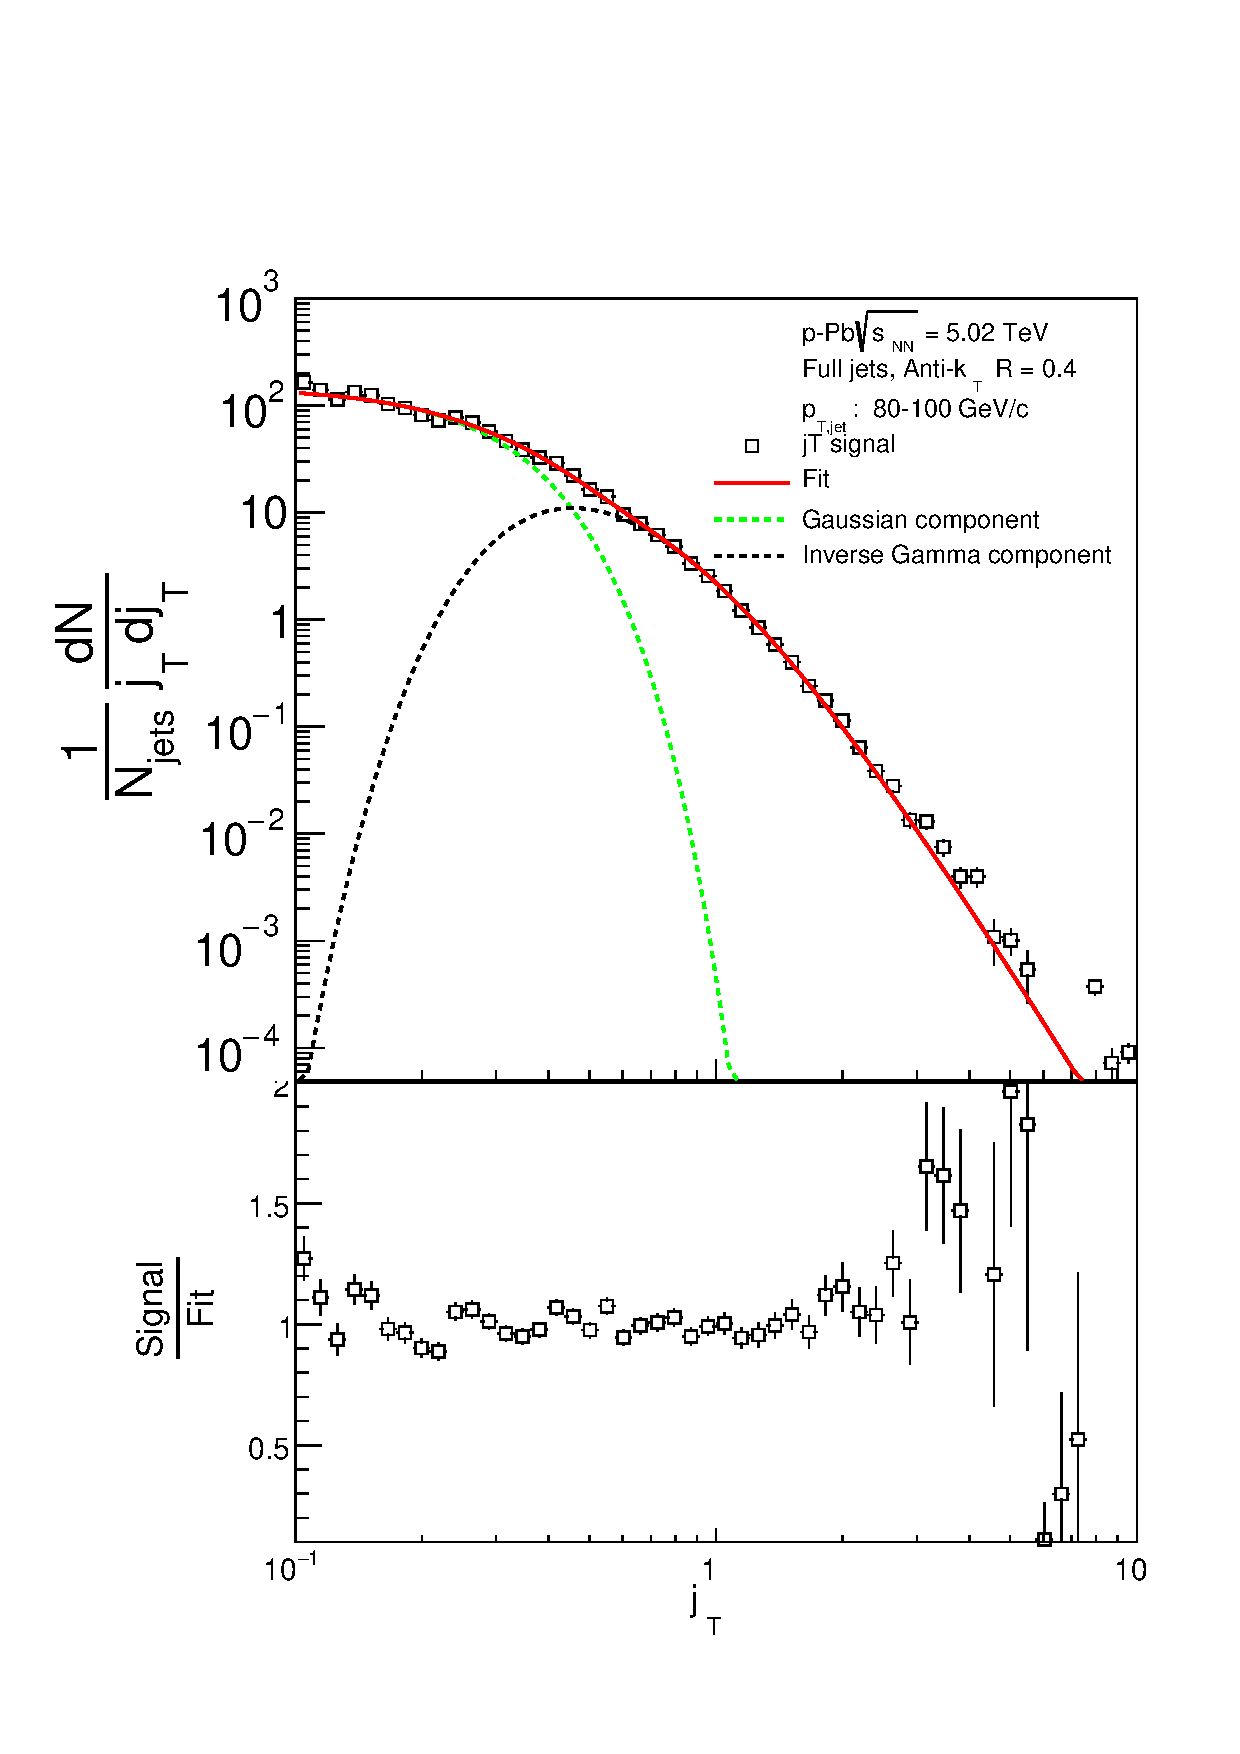
\includegraphics[width=0.95\textwidth]{results/JetConejTSignalFit/JetConejTSignalFitNFin00JetPt06perconeBgBayes}
\end{subfigure}
\begin{subfigure}{0.24\textwidth}
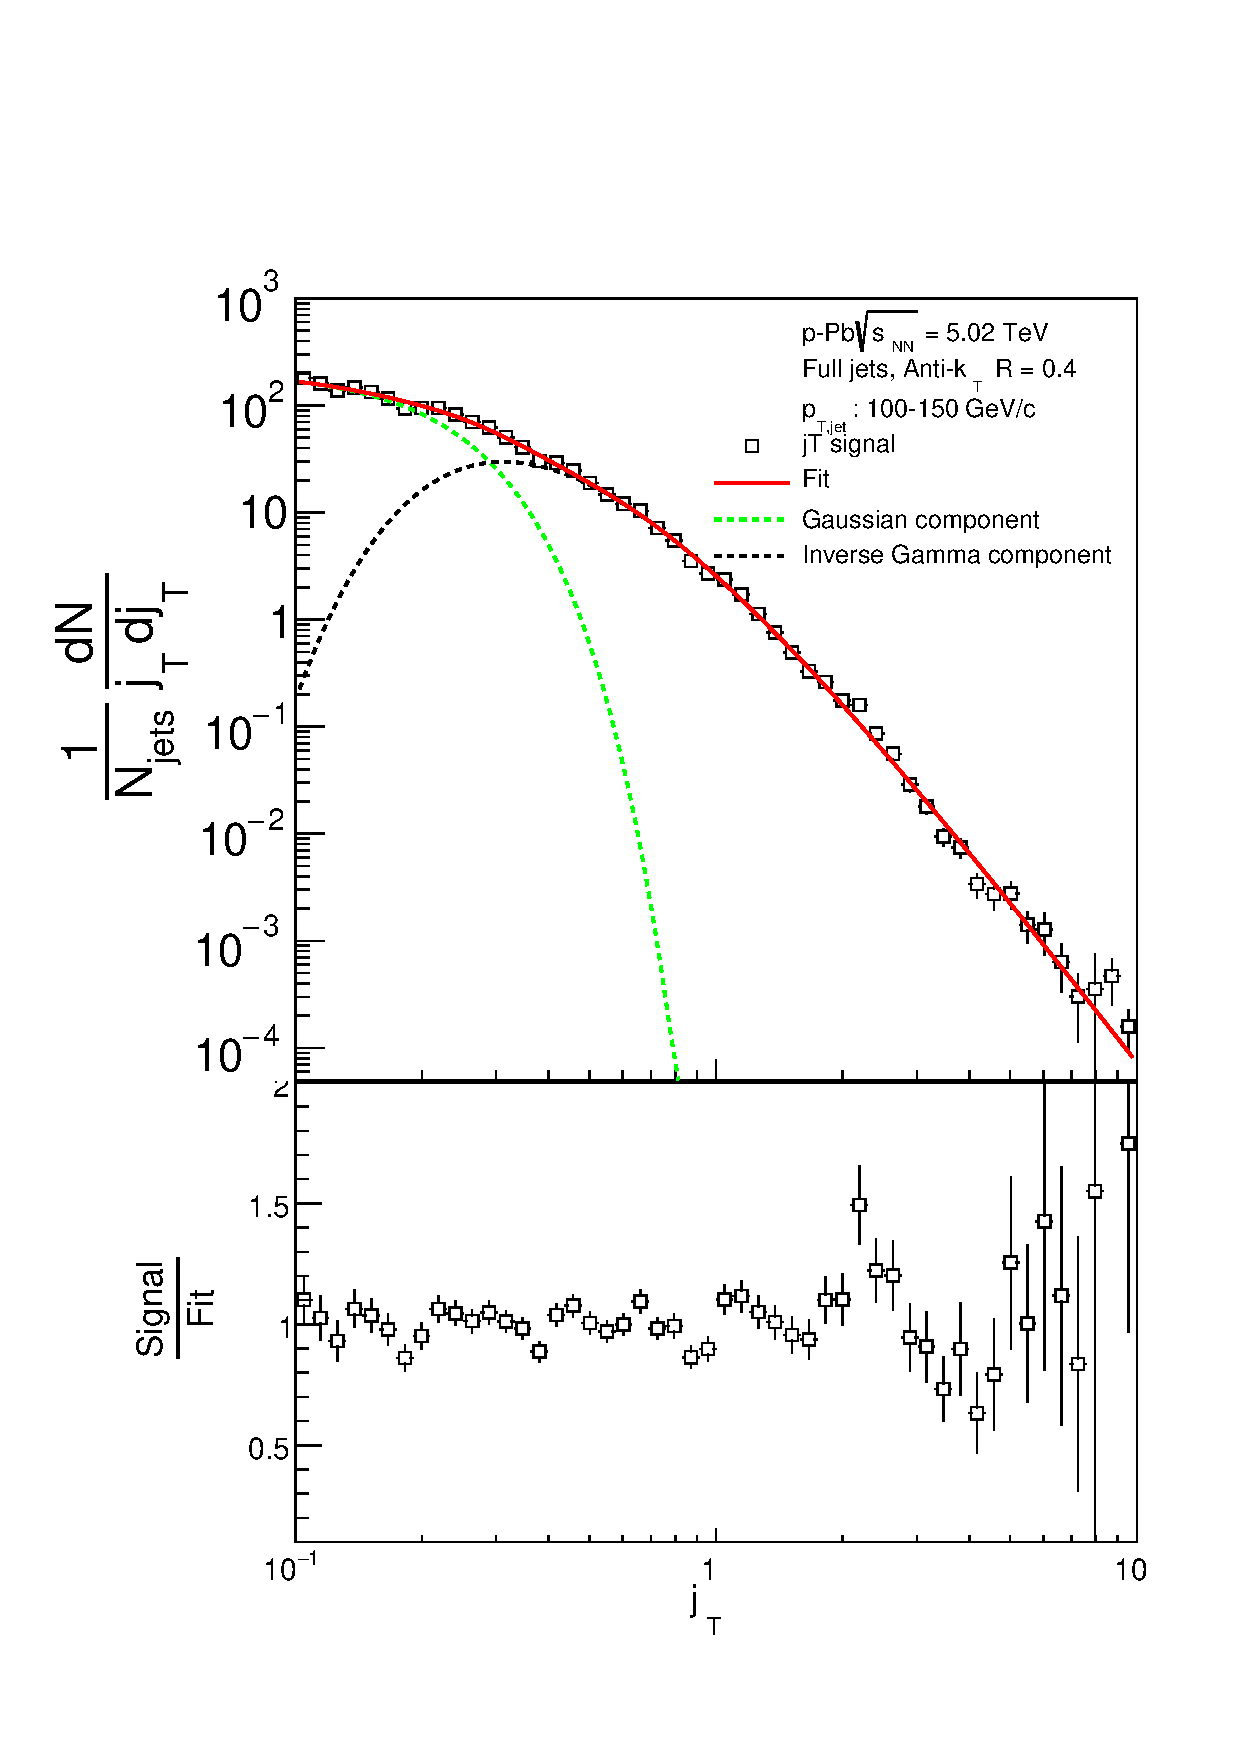
\includegraphics[width=0.95\textwidth]{results/JetConejTSignalFit/JetConejTSignalFitNFin00JetPt07perconeBgBayes}
\end{subfigure}
\caption{$j_T$ signal fits in different jet $p_T$ bins}
\label{fig:fits}
\end{figure}




\subsubsection{RMS values from fitted distributions}
RMS results with systematic errors are shown separately in figure \ref{fig:rmsyield}. Figure \ref{fig:rms} shows RMS values for both components combined. The figure also includes results from a PYTHIA simulation. 
\begin{figure}[htb]
\begin{subfigure}{0.5\textwidth}
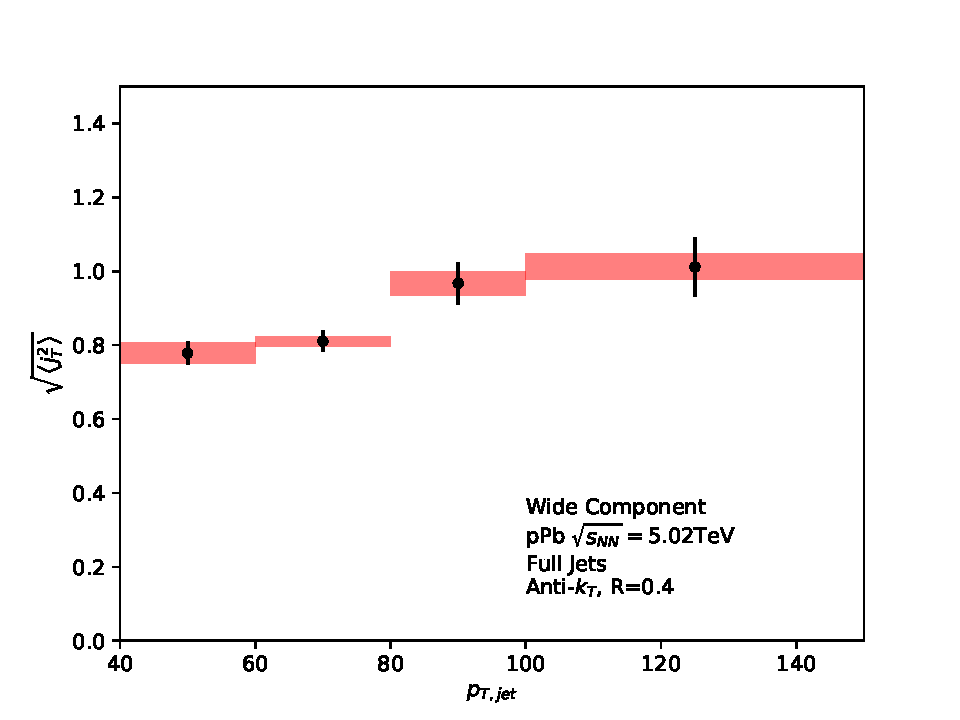
\includegraphics[width=0.95\textwidth]{results/gammaRMSWithSystematics}
\end{subfigure}
%\begin{subfigure}{0.5\textwidth}
%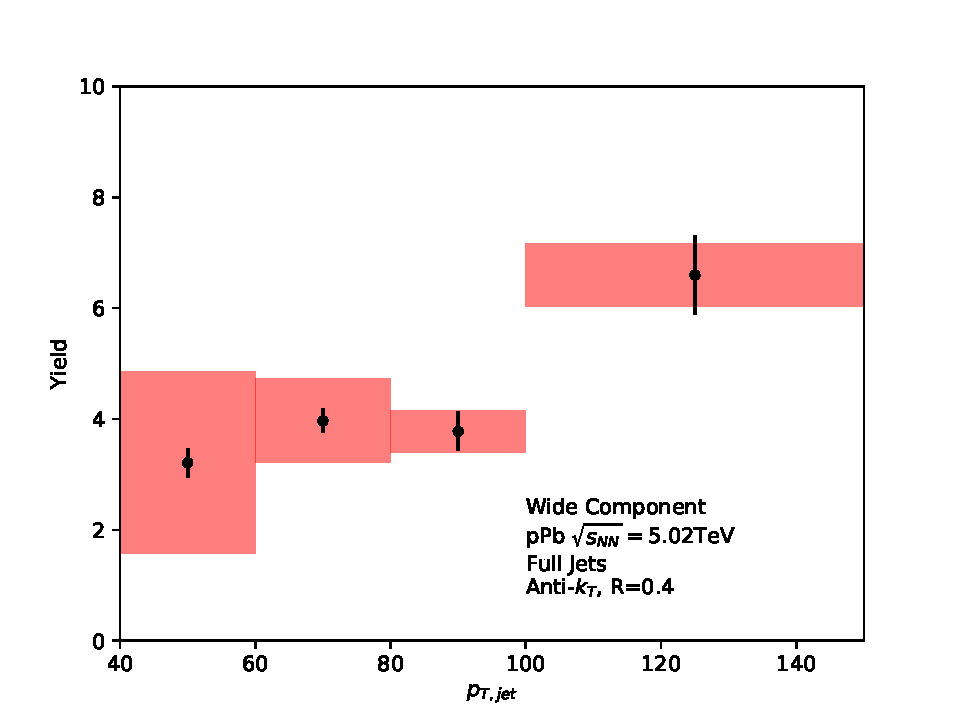
\includegraphics[width=0.95\textwidth]{results/gammaYieldWithSystematics}
%\end{subfigure}
\begin{subfigure}{0.5\textwidth}
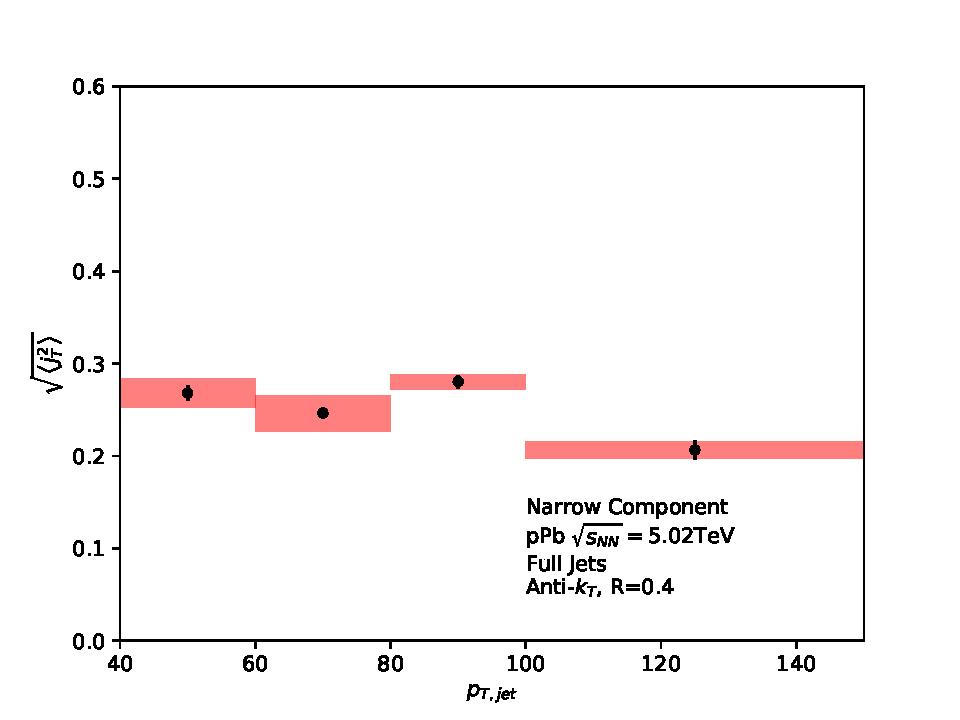
\includegraphics[width=0.95\textwidth]{results/gausRMSWithSystematics}
\end{subfigure}
%\begin{subfigure}{0.5\textwidth}
%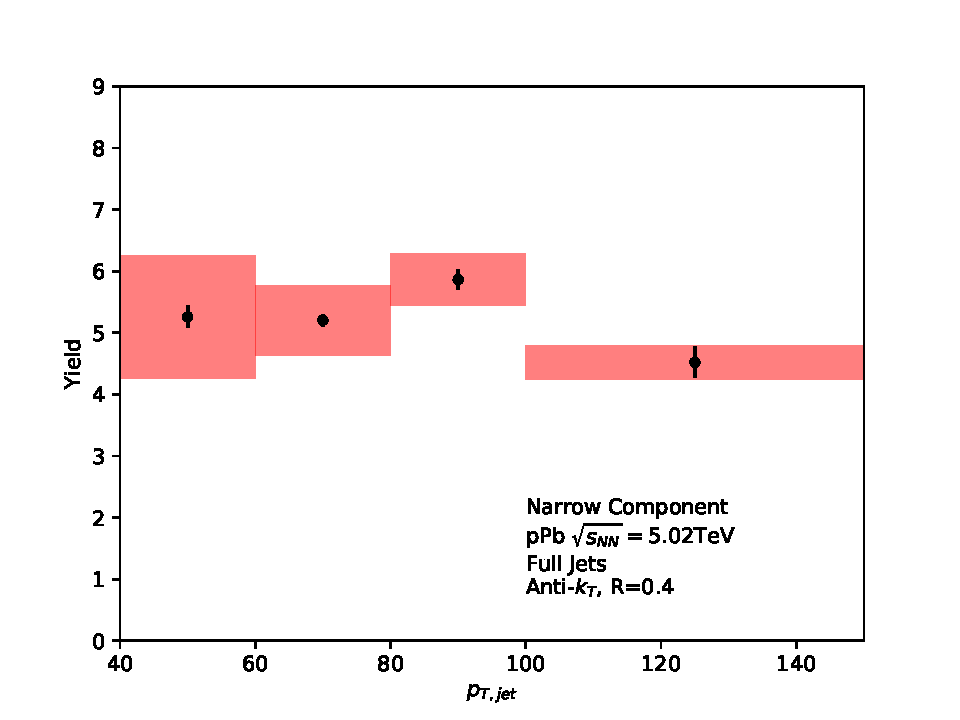
\includegraphics[width=0.95\textwidth]{results/gausYieldWithSystematics}
%\end{subfigure}
\caption{RMS values extracted from the fits for the gaussian (narrow) and inverse gamma (wide) components}
\label{fig:rmsyield}
\end{figure}

\begin{figure}[htb]
\begin{subfigure}{0.5\textwidth}
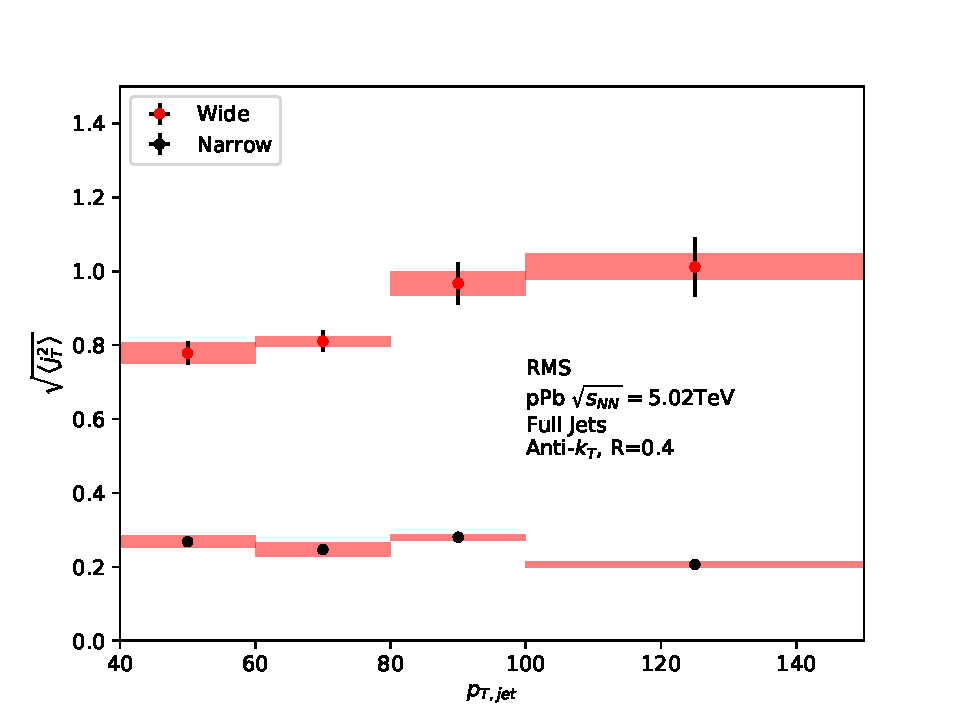
\includegraphics[width=0.95\textwidth]{results/RMSWithSystematics}
\end{subfigure}
\begin{subfigure}{0.5\textwidth}
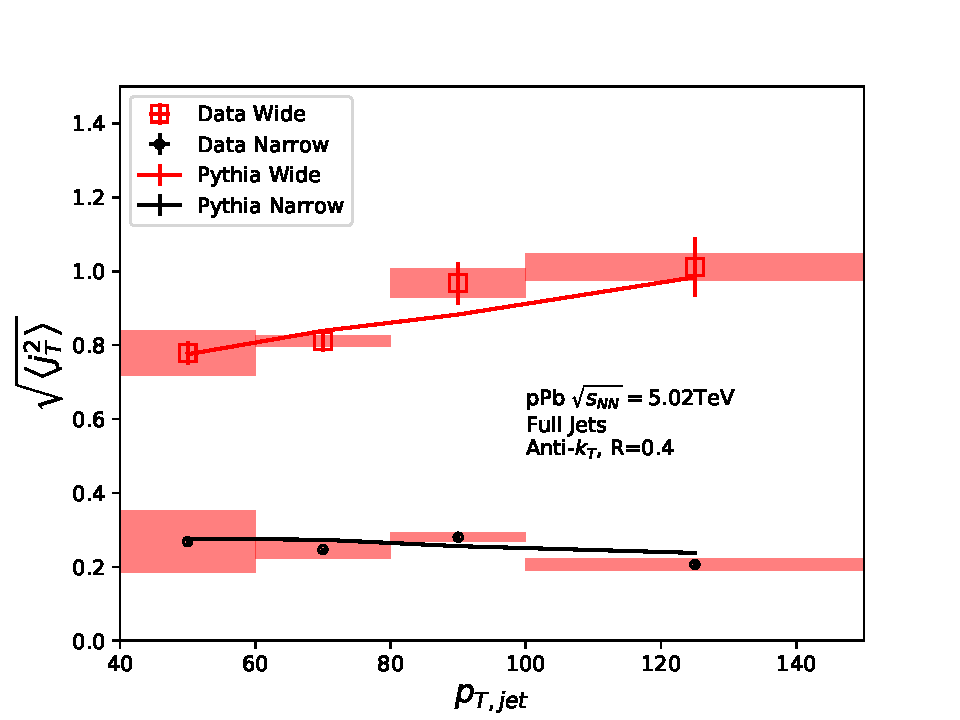
\includegraphics[width=0.95\textwidth]{results/RMSWithSystematics_Pythia}
\end{subfigure}
\caption{RMS values extracted from the fits for the gaussian (narrow) and inverse gamma (wide) components}
\label{fig:rms}
\end{figure}

\subsection{High multiplicity}
The analysis was repeated taking only events with high multiplicity. Three different multiplicity cuts were used; \unit[10]{\%}, \unit[1]{\%} and \unit[0.1]{\%}. We used ZDC(TODO) as a centrality estimator. As argued in section ~\ref{sec:} the zero-degree energy deposit should provide a centrality estimator with minimal bias from jets production. Resulting $\jt{}$ distributions are shown Fig.~\ref{fig:highm}. As the statistics are limited in the high multiplicity runs, it was hard to achieve stable fits to the distributions, thus the RMS values are not shown.

From the figure one can observe no systematic modification when tighter multiplicity cuts are introduced. 

\begin{figure}[htb]
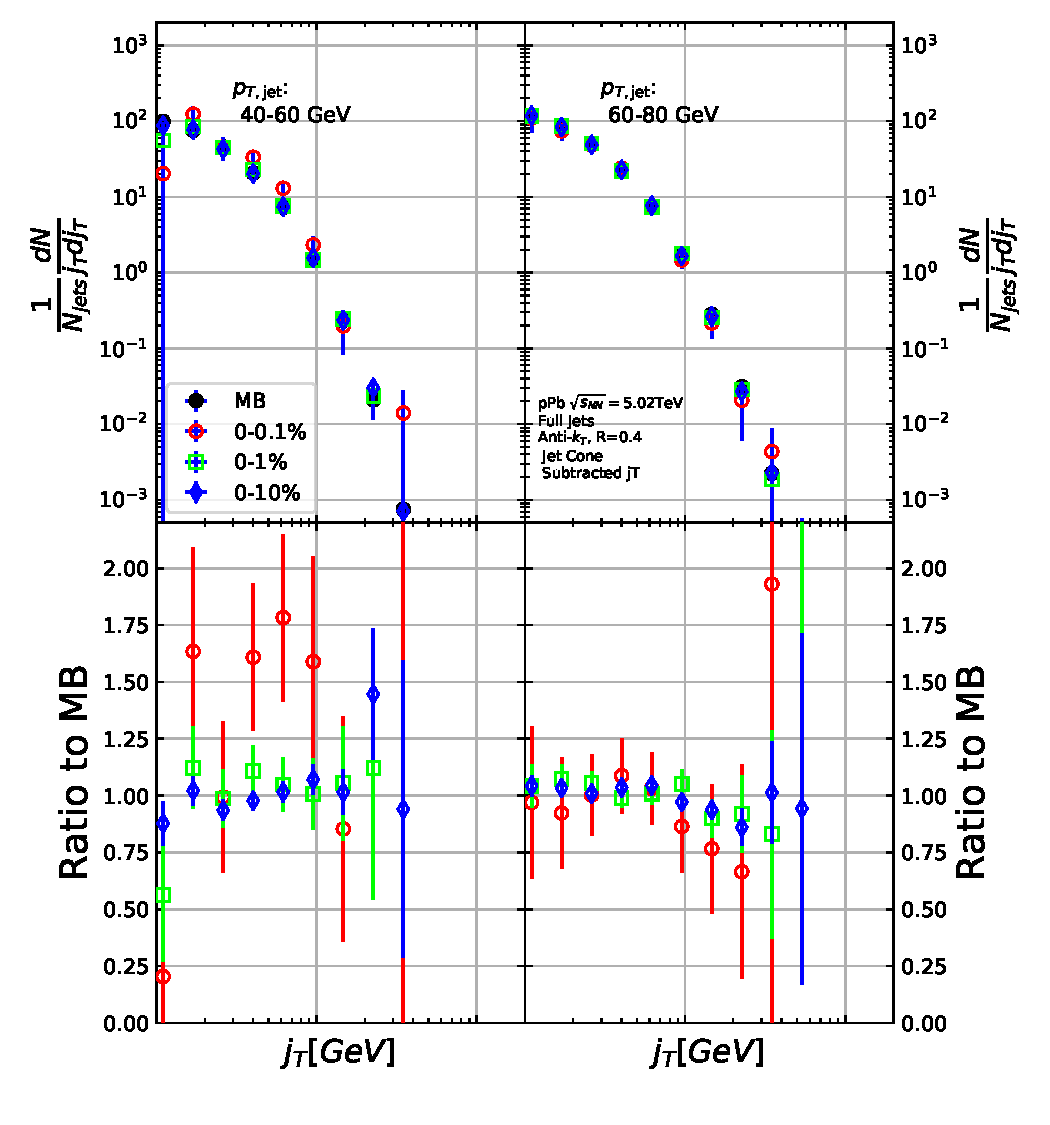
\includegraphics[width=0.95\textwidth]{results/HighMJetConeJtSignalPtFrom3To8.pdf}
\caption{$\jt{}$ distributions for high multiplicity \pPb~ events }
\label{fig:highm}
\end{figure}



